\documentclass[a4paper, 12pt]{article}
\usepackage{graphicx}
\usepackage[margin=2cm]{geometry}
\usepackage[hidelinks]{hyperref}
\usepackage[croatian]{babel}
\usepackage[sorting=none]{biblatex}
    \addbibresource{ref.bib}
\usepackage{float}


% Boje za kod:
\usepackage{xcolor,graphicx}
\usepackage{listings}

\definecolor{solarized-base03}{RGB}{0, 43, 54}
\definecolor{solarized-base02}{RGB}{7, 54, 66}
\definecolor{solarized-base01}{RGB}{88, 110, 117}
\definecolor{solarized-base00}{RGB}{101, 123, 131}
\definecolor{solarized-base0}{RGB}{131, 148, 150}
\definecolor{solarized-base1}{RGB}{147, 161, 161}
\definecolor{solarized-base2}{RGB}{238, 232, 213}
\definecolor{solarized-base3}{RGB}{253, 246, 227}
\definecolor{solarized-yellow}{RGB}{181, 137, 0}
\definecolor{solarized-orange}{RGB}{203, 75, 22}
\definecolor{solarized-red}{RGB}{220, 50, 47}
\definecolor{solarized-magenta}{RGB}{211, 54, 130}
\definecolor{solarized-violet}{RGB}{108, 113, 196}
\definecolor{solarized-blue}{RGB}{38, 139, 210}
\definecolor{solarized-cyan}{RGB}{42, 161, 198}
\definecolor{solarized-green}{RGB}{133, 153, 0}

\lstset{
  basicstyle=\footnotesize\ttfamily\color{solarized-base00},
  keywordstyle=\color{solarized-blue}\bfseries,
  commentstyle=\color{solarized-base1},
  stringstyle=\color{solarized-cyan},
  identifierstyle=\color{solarized-violet},
  numberstyle=\tiny\color{solarized-base01},
  numbers=left,
  firstnumber=1,
  stepnumber=1,
  showstringspaces=false,
  tabsize=4,
  frame=none,
  framerule=1pt,
  framexleftmargin=5pt,
  framexrightmargin=5pt,
  framextopmargin=3pt,
  framexbottommargin=3pt,
  backgroundcolor=\color{solarized-base3},
  rulecolor=\color{solarized-base01},
  breaklines=true,
  breakatwhitespace=true,
  language=C++
}


\begin{document}
\noindent
Univerzitet u Sarajevu\\
Elektrotehnički fakultet\\
Predmet: Uvod u digitalnu obradu slike\\
Predmetni profesor: prof. dr Emir Sokić\\
Autor: Berina Biberović\\
Akademska godina: 2022/2023.


\begin{center}
    \section*{Tutorijal 2}
    \subsection*{Pikseli unutar slike. Prostori boja.}
\end{center}


\subsection*{Manipulacija tačkama/koordinatama}

Važan dio obrade slike je mogućnost pristupanja pojedinačnim pikselima unutar učitane slike. Za te svrhe unutar OpenCV-a postoje posebne klase koje nam omogućavaju upravo to.

\subsubsection*{\lstinline{template<typename _Tp> class cv::Point_<_Tp>} klasa}

Klasa \lstinline{template<typename _Tp> class cv::Point_<_Tp>} je šablonska klasa za 2D tačke koja je opisana svojim koordinatama $x$ i $y$. Ovdje, kao što se može pretpostaviti, varijabla unutar šablona \lstinline{_Tp} može biti tipa \lstinline{int}, \lstinline{double}, \lstinline{float}. Dakle, ukoliko npr. želimo napraviti instancu ove klase gdje su koordinate tipa \lstinline{int}, onda možemo pisati:

\begin{lstlisting}
    cv::Point_<int> tacka(3, 5);
\end{lstlisting}

Ova klasa se nalazi unutar \lstinline{core} modula, preciznije unutar \lstinline{core/types.hpp}. Bitno je istaći da postoji cast operator koji konvertuje automatski koordinate u specificirani tip. Konverzija iz decimalnih tipova u cjelobrojne se radi preko zaokruživanja. Isto tako, postoje još definirane operacije koje su dozvoljene da se rade nad \lstinline{template<typename _Tp> class cv::Point_<_Tp>} tipovima, koje možete naći na \href{https://docs.opencv.org/3.4/db/d4e/classcv_1_1Point__.html}{ovom linku} (kao i još neke detalje o \lstinline{template<typename _Tp> class cv::Point_<_Tp>} klasi).

\subsubsection*{\lstinline{template<typename _Tp> class cv::Point3_<_Tp>} klasa}

Slično kao prethodno spomenuta klasa, \lstinline{template<typename _Tp>  class cv::Point3_<_Tp>} klasa je šablonska klasa koja je specificirana sa tri koordinate $x$, $y$ i $z$. Kao i u prethodnoj klasi, koordinate 3D tačaka se mogu konvertovati u drugi tip. Vektorska aritmetika i operacije upoređivanja su podržane za ovu klasu. Na sličan način se incijaliziraju instance ove klase kao i prethodne, samo što je potrebno proslijediti tri parametra umjesto dva. Detalje možete pronaći na \href{https://docs.opencv.org/3.4/df/d6c/classcv_1_1Point3__.html}{ovom linku}.

\subsubsection*{Pristupanje pikselima unutar objekata klase \lstinline{cv::Mat}}

Da bismo mogli pristupiti vrijednosti piksela unutar slike moramo znati tip slike i broj kanala. Postoji više tipova slike, kao što su binarne, \textit{grayscale}, indeksirane, RGB, itd. Ovaj tutorijal će preći kako pristupiti pikeslima jednokanalne \textit{grayscale} slike i RGB trokanalne slike. 

Da bi se pristupilo pikselu sa koordinatama $x$ i $y$ unutar jednokanalne \textit{grayscale} slike, potrebno je napisati:

\begin{lstlisting}
cv::Scalar intenzitet = slika.at<uchar>(y, x);
\end{lstlisting}

Klasa \lstinline{cv::Scalar} je šablonska klasa (\lstinline{template<typename _Tp> class Scalar_<double>}) koja se nalazi unutar \lstinline{core/types.hpp} modula. Ova klasa je derivirana iz klase \lstinline{cv::Vec} (nećemo se baviti detaljima \lstinline{cv::Vec} klase) i predstavlja 4-elementni vektor. Instance ove klase se mogu koristiti kao tipični 4-elementni vektori i mogu se konvertovati iz i u \lstinline{cv::CvScalar} tip. Tip \lstinline{cv::Scalar} se široko koristi u OpenCV-u kako bi se vrijednosti piksela mogli čitati i pisati.

Tip \lstinline{uchar} je samo \lstinline{typedef unsigned char uchar} (dakle, vrijednost intenziteta piksela ne može biti negativna u ovom kontekstu!).

Unutar C++ jezika \lstinline{intenzitet.val[0]} sadrži vrijednost od 0 do 255. Potrebno je obratiti pažnju na redoslijed koordinata $x$ i $y$ - kako su u OpenCV-u slike predstavljene kao ista struktura kao što su matrice, onda se ista konvencija koristi za oba slučaja: $y$ koordinata predstavlja red matrice, dok $x$ koordinata predstavlja kolonu matrice. Alternativno, može se pisati i:

\begin{lstlisting}
cv::Scalar intenzitet = slika.at<uchar>(cv::Point(x, y));
\end{lstlisting}

Da bismo pristupili pikselu sa $x$ i $y$ koordinatama unutar trokanalne BGR slike (podrazumijevani format koji se učitava svaki put kada koristimo \lstinline{cv::imread}) trebamo pisati:

\begin{lstlisting}
cv::Vec3b intenzitet = slika.at<cv::Vec3b>(cv::Point(x, y));
uchar plava = intenzitet.val[0];
uchar zelena = intenzitet.val[1];
uchar crvena = intenzitet.val[2];
\end{lstlisting}

Klasa \lstinline{cv::Vec3b} se nalazi unutar modula \lstinline{core/matx.hpp} i nasljđena je iz prethodno spomenute klase \lstinline{cv::Vec}, koja u ovom slučaju predstavlja 3-elementni vektor čiji su elementi tipa \lstinline{uchar}. Alternativno, može se ista metoda iskoristiti za \textit{floating point} slike (koje se mogu dobiti npr. kada se Sobel transformacija uradi nad trokanalnom slikom) ako se umjesto \lstinline{cv::Vec3b} u prethodnom isječku koda piše \lstinline{cv::Vec3f}.

U prethodnom isječku koda, svaka od vrijednosti \lstinline{vrijednost.val[0]}, \lstinline{vrijednost.val[1]} i \lstinline{vrijednost.val[2]} mogu biti od 0 do 255. Primjetimo da, iako u govoru ove slike nazivamo RGB slikama, redoslijed unutar OpenCV-a nije RGB, nego BGR (veoma važno je paziti na taj redoslijed u toku testova, jer mnoge greške se naprave tu).

Postoje još neke metode koje se mogu raditi nad pikselima slika i različiti načini na koji se oni mogu predstavljati, ali u ovom tutorijalu nećemo više obrađivati tu temu, nego u budućim tutorijalima ako bude bilo potrebe za tim. 

\subsection*{Prostori boja}

Prostori boja (eng. \textit{color spaces}) predstavljaju specifičan način organizacije boja. Neki prostor boja podržava reproducibilne reprezentacije boja - bile one u analgonom ili digitalnom formatu. Model boje (eng. \textit{color model}) je apstraktni matematički model koji opisuje način na koji boje mogu biti predstavljene kao n-torke brojeva. Ukoliko dodamo specifičnu funkciju mapiranja između modela boje i referentnog prostora boje postižemo unutar referentnog prostora boje definitivni "otisak" (tzv. gamut) i za dati model boje ovo definira prostor boje. Kako prostor boja inače znači određenu kombinaciju modela boje i funkcije mapiranja, prostor boje se inače koristi kao sinonim za model boje, ali ovo korištenje je netačno u strogom obliku. Npr. iako postoje više specifičnih prostora boja koji se zasnivaju na RGB modelu boje, ne postoji singularni RGB prostor boje.

\subsubsection*{Konverzije prostora boja}

Na predavanju 2 je bilo spomenuto nekoliko prostora boja kao što su npr. RGB, CMY i CMYK, Lab, HSV, HSL, itd. Pored toga, na predavanju 2 su navedene funkcije konverzije iz jednog prostora boja u drugi. Unutar C++ mi možemo definirati naše funkcije koje bi radile konverzije onako kako su one navedene na predavanju, ali, srećom OpenCV nam omogućava da ne moramo te konverzije raditi "ručno", već postoje funkcije koje automatski rade konverziju za nas. 

Unutar OpenCV-a, da bismo konvertovali sliku iz jednog u drugi prostor boje, možemo koristiti funkciju \lstinline{cv::cvtColor(InputArray izvorna_slika, OutputArray destinacijska_slika, int kod, int br_kan = 0)}: parametar \lstinline{izvorna_slika} predstavlja sliku (8-bitna unsigned, 16-bitna unsigned ili single-precision floating point) koju želimo prebaciti u novi prostor boja; parametar \lstinline{destinacijska_slika} je rezultantna slika obrade konverzije koja mora biti iste veličine i dubina kao \lstinline{izvorna_slika}; \lstinline{kod} predstavlja konverzijski kod prostora boja (listu možete naći \href{https://docs.opencv.org/3.4/d8/d01/group__imgproc__color__conversions.html}{ovdje}); a \lstinline{br_kan} predstavlja broj kanala u rezultantnoj slici - ukoliko je taj parametar jednak 0, onda broj kanala se automatski očitava iz \lstinline{izvorna_slika} i \lstinline{kod}. Ova funkcija se nalazi unutar modula \lstinline{imgproc.hpp}, tako da je potrebno taj modul uključiti na početku programa.

Slijedi jednostavan primjer učitavanja BGR slike, prebacivanja je u \textit{grayscale}, HSV i binarnu sliku.

\begin{lstlisting}
#include <opencv4/opencv2/core/mat.hpp>
#include <opencv4/opencv2/highgui.hpp>
#include <opencv4/opencv2/imgcodecs.hpp>
#include <opencv4/opencv2/imgproc.hpp>

int main() {

    // Ucitavanje BGR slike:
    cv::Mat BGR_slika = cv::imread("/home/anniberi/Pictures/Wallpapers/cat.jpeg", cv::IMREAD_COLOR);

    // Deklarisanje grayscale, binarne i HSV slike:
    cv::Mat gray_slika, bin_slika, HSV_slika;

    // Koristenje cv::cvtColor funkcije kako bismo dobili grayscale i HSV sliku:
    cv::cvtColor(BGR_slika, gray_slika, cv::COLOR_BGR2GRAY);
    cv::cvtColor(BGR_slika, HSV_slika, cv::COLOR_BGR2HSV);

    // Koristenje threshold funkcije kako bismo dobili binarnu sliku:
    cv::threshold(gray_slika, bin_slika, 120, 255, cv::THRESH_BINARY);

    // Prikaz svih slika:
    cv::imshow("BGR slika", BGR_slika);
    cv::imshow("Grayscale slika", gray_slika);
    cv::imshow("HSV slika", HSV_slika);
    cv::imshow("Binarna slika", bin_slika);

    cv::waitKey();

    return 0;
}
\end{lstlisting}

Možemo primijetiti da, kako bismo sliku prebacili iz \textit{grayscale} u binarnu nismo koristili funkciju \lstinline{cv::cvtColor} nego smo koristili funkciju \lstinline{cv::threshold}. Ova funkcija prima 5 parametara: ulaznu \textit{grayscale sliku}; izlaznu sliku koja će biti rezultat pretvaranja ulazne slike u binarnu sliku; parametar tip \lstinline{double} koji predstavlja prag intenziteta piksela gdje sve manje od tog praga predstavlja 0, a sve veće od njega predstavlja 1; parametar tipa \lstinline{double} koji predstavlja maksimalnu vrijednost koja se koristi sa \textit{thresholding} \lstinline{enum} tipovima \lstinline{cv::THRESH_BINARY} i \lstinline{cv::THRESH_BINARY_INV}; i na kraju parametar tipa \lstinline{int} koji predstavlja upravo \lstinline{enum} \textit{thresholding} tip.

Još jedan tip \textit{thresholding}-a koji postoji je adaptivni thresholding kojeg ćemo pokazati na jednostavnom primjeru.

\begin{lstlisting}
#include <opencv4/opencv2/core/mat.hpp>
#include <opencv4/opencv2/imgproc.hpp>
#include <opencv4/opencv2/imgcodecs.hpp>
#include <opencv4/opencv2/highgui.hpp>

int main() {

    // Ucitavnanje slike u grayscale-u:
    cv::Mat slika = cv::imread("/home/anniberi/Pictures/Wallpapers/cat.jpeg", cv::IMREAD_GRAYSCALE);
    cv::Mat binarna;

    // Pravljenje trackbar-ova:
    cv::namedWindow("Trackbars");
    cv::createTrackbar("Threshold 1", "Trackbars", nullptr, 255);
    cv::createTrackbar("(Block size - 3) / 2", "Trackbars", nullptr, 255);
    cv::namedWindow("Adaptivni thresholding");
    cv::namedWindow("Originalna grayscale slika");

    int t1, t2;

    do {

        // Ucitavanje t1 i t2 sa trackbarova:
        t1 = cv::getTrackbarPos("Threshold 1", "Trackbars");
        t2 = cv::getTrackbarPos("(Block size - 3) / 2", "Trackbars");

        // Sada primjenjujemo funkciju za adaptivni thresholding:
        cv::adaptiveThreshold(slika, binarna, 255, cv::ADAPTIVE_THRESH_MEAN_C, cv::THRESH_BINARY, 2 * t2 + 3, t1);
        // Prikaz slika:
        cv::imshow("Originalna grayscale slika", slika);
        cv::imshow("Adaptivni thresholding", binarna);

    }while(cv::waitKey() != 'q');

    cv::destroyAllWindows();

    return 0;
}
\end{lstlisting}

U gornjem kodu smo iskoristili da originalnu sliku odmah učitamo u \textit{grayscale} tipu, koristeći parametar \lstinline{cv::IMREAD_GRAYSCALE} unutar funkcije \lstinline{cv::imread}. Nakon toga smo korištenjem funkcije \lstinline{cv::namedWindow} napravili prozor pod imenom "Trackbars" u kojem ćemo staviti \textit{trackbar}-ove koji će nam koristiti za adaptivni \textit{thresholding}. Funkcija \lstinline{cv::createTrackbar} prima 6 parametara: prvi parametar je tipa \lstinline{const String &} i predstavlja ime koje dajemo specifičnom \textit{trackbar}-u; drugi parametar je isto tipa \lstinline{const String &} i predstavlja ime prozora kojeg smo kreirali u prethodnoj liniji koda; treći parametar je tipa \lstinline{int*} i predstavlja pokazivač na cjelobrojnu varijablu čija vrijednost reflektuje poziciju \textit{slider}-a i prilikom kreiranja pozicija \textit{slider}-a se definira preko ove varijable (u našem slučaju je to \lstinline{nullptr} tako da ne pokazuje ni na šta na početku, ali to je ok jer mi možemo pomjerati \textit{slider} lijevo-desno); četvrti parametar je tipa \lstinline{int} i predstavlja maksimalnu poziciju do koje može ići \textit{slider} - kod nas je to 255; zadnja dva parametra su predefinirana i predstavljaju tipove \lstinline{cv::TrackbarCallback} i \lstinline{void *} koji su postavljeni automatski na 0 pri pozivanju funkcije.

Nakon što smo napravili dva ista \textit{trackbar}-a sa različitim imenima unutar istog prozora, pravimo još dva prozora - za \textit{grayscale} sliku i za sliku koju mijenjamo adaptivnim \textit{thresholding}-om. Deklarišemo onda dvije varijable koje će nam služiti za uzimanje trenutne vrijednosti oba \textit{trackbar}-a - \lstinline{t1} i \lstinline{t2}. 

Unutar \lstinline{do while} petlje učitavamo vrijednosti u \lstinline{t1} i \lstinline{t2} preko funkcije \lstinline{cv::getTrackbarPos} koja prima dva parametra - ime \textit{trackbar}-a kojeg želimo pročitati i ime prozora u kojem se taj \textit{trackbar} nalazi. 

Onda primjenjujemo funkciju \lstinline{cv::adaptiveThreshold} koja prima 7 parametara: prvi parametar je ulazna \textit{grayscale} slika; drugi parametar je izlazna binarna slika; treći parametar je tipa \lstinline{double} i predstavlja nenultu vrijednost koja se daje pikselima za koje je uslov ispunjen; četvrti parametar je tipa \lstinline{int} i predstavlja koji algoritam se treba koristiti za adaptivni \textit{thresholding}; peti parametar je tipa \lstinline{int} i predstavlja \textit{thresholding} tip koji mora biti ili \lstinline{cv::THERSH_BINARY} ili \lstinline{cv::THRESH_BINARY_INV}; šesti parametar je isto tipa \lstinline{int} i predstavlja veličinu susjedstva piksela koja se koristi da bi se izračunala \textit{threshold} vrijednost za piksel; sedmi parametar je tipa \lstinline{double} i predstavlja konstantu koja se oduzima od srednje vrijednosti. Više detalja možete pronaći na \href{https://docs.opencv.org/3.4/d7/d1b/group__imgproc__misc.html#ga72b913f352e4a1b1b397736707afcde3}{linku}.

Nakon toga unutar odgovarajućih prozora prikazujemo \textit{grayscale} sliku i sliku koju smo dobili kroz \textit{thresholding}. Na slici \ref{sl1} je prikazana originalna \textit{grayscale} slika, dok je na slici \ref{sl2} prikazana slika nakon primjenjivanja adaptivnog \textit{thresholding}-a. Studentima se savjetuje da prođu kroz sve primjere sa tutorijala i sami probaju ubaciti neke svoje slike u program i vide šta se dešava sa slikama koje su na ovaj način promijenili.

\begin{figure}[H]
    \minipage{0.49\textwidth}
        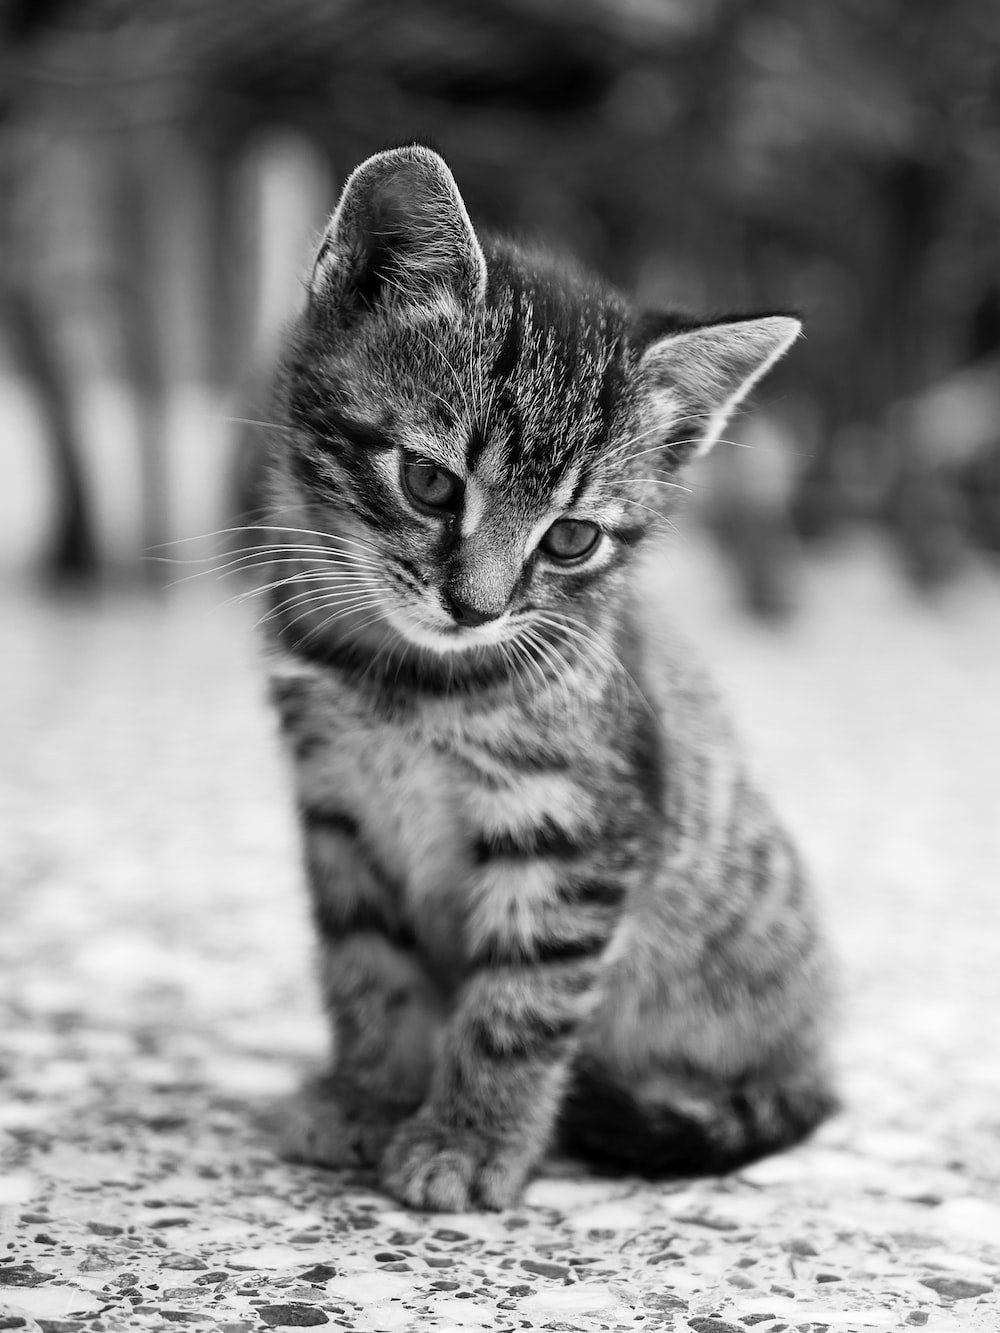
\includegraphics[width=\linewidth]{Slike/originalna.jpg}
        \caption{Originalna \textit{grayscale} slika}\label{sl1}
    \endminipage\hfill
    \minipage{0.49\textwidth}
        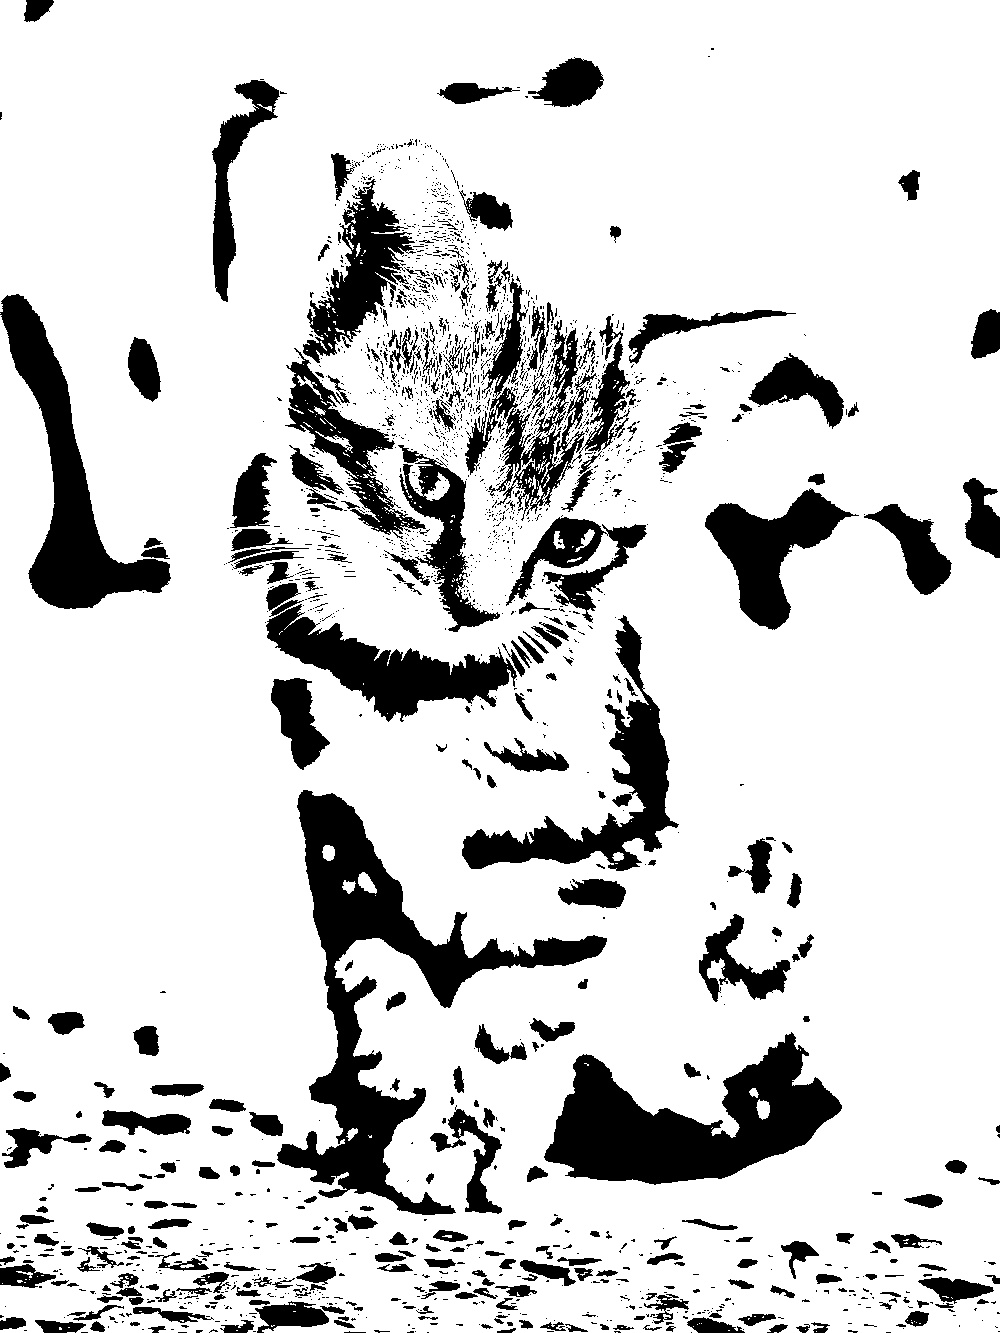
\includegraphics[width=\linewidth]{Slike/binarna.jpg}
        \caption{Binarna slika nakon \textit{thresholding}-a}\label{sl2}
    \endminipage\hfill
\end{figure}

\subsection*{Napomene}

Korištena tema za prikaz C++ koda na tutorijalima je \href{https://ethanschoonover.com/solarized/}{\lstinline{solarized}}\cite{solarized}.

\printbibliography

\end{document}
